\section{Example}\label{sec:example}
\mkAgenda
\begin{frame}{Example}
    \begin{columns}
        \begin{column}{0.65\textwidth}
            \begin{itemize}
                \item<+-> Naive matrix multiply
                \item<+-> Each element in $C$ is independently computed
                \item<+-> Steps:
                \begin{enumerate}
                    \item<.-> Starting C++ code
                    \item<+-> Allocate GPU memory
                    \item<+-> Copy $A$, $B$ to GPU
                    \item<+-> Start kernel (using $m \cdot p$ GPU threads)
                    \item<+-> Copy $C$ to CPU
                \end{enumerate}
            \end{itemize}
        \end{column}
        \begin{column}{0.3\textwidth}
            \resizebox{0.95\linewidth}{!}{\newcommand{\smArr}{{Latex[length=0.5mm,width=0.5mm]}}
\begin{tikzpicture}
    % Background & grid
    \fill[blue!20!white] (-1.201,-1.501) rectangle (0,0);
    \draw[step=0.1cm,blue,very thin] (-1.201,-1.501) grid (0,0);
    % Central letter
    \draw (-0.6,-0.75) node[anchor=center,text=Blue] {{\Huge $A$}};
    % Selected row
    \draw[blue,rounded corners=0.05cm] (-1.2125,-0.1125) rectangle (0.0125,0.0125);
    \draw[-\smArr,blue] (0.0125,-0.05) -- (0.0875,-0.05);
    % Dimensions
    \draw[\smArr-\smArr,blue,anchor=center] (-1.3,-1.501) -- (-1.3,0);
    \draw (-1.45,-0.75) node[anchor=center,text=blue] {{\tiny $m$}};
    \draw[\smArr-\smArr,blue,anchor=center] (-1.201,-1.6) -- (0,-1.6);
    \draw (-0.6,-1.75) node[anchor=center,text=blue] {{\tiny $n$}};

    % Background & grid
    \fill[red!20!white] (0.1,0.1) rectangle (1.1,1.3);
    \draw[step=0.1cm,red,very thin] (0.1,0.1) grid (1.1,1.3);
    % Central letter
    \draw (0.6,0.7) node[anchor=center,text=BrickRed] {{\Huge $B$}};
    % Selected row
    \draw[BrickRed,rounded corners=0.05cm] (0.0875,0.0875) rectangle (0.2125,1.3125);
    \draw[-{Latex[length=0.5mm,width=0.5mm]},BrickRed] (0.15,0.0875) -- (0.15,0.0125);
    % Dimensions
    \draw[\smArr-\smArr,BrickRed,anchor=center] (1.2,0.1) -- (1.2,1.3);
    \draw (1.35,0.7) node[anchor=center,text=BrickRed] {{\tiny $n$}};
    \draw[\smArr-\smArr,BrickRed,anchor=center] (0.1,1.4) -- (1.1,1.4);
    \draw (0.6,1.55) node[anchor=center,text=BrickRed] {{\tiny $p$}};

    % Background & grid
    \fill[green!20!white] (0.1,-1.505) rectangle (1.1,0);
    \draw[step=0.1cm,OliveGreen,very thin] (0.1,-1.505) grid (1.1,0);
    % Central letter
    \draw (0.6,-0.75) node[anchor=center,text=OliveGreen] {{\Huge $C$}};
    % Selected cell
    \draw[OliveGreen,rounded corners=0.05cm] (0.0875,-0.1125) rectangle (0.2125,0.0125);
    % Dimensions
    \draw[\smArr-\smArr,OliveGreen,anchor=center] (1.2,0) -- (1.2,-1.505);
    \draw (1.35,-0.75) node[anchor=center,text=OliveGreen] {{\tiny $m$}};
    \draw[\smArr-\smArr,OliveGreen,anchor=center] (0.1,-1.6) -- (1.1,-1.6);
    \draw (0.6,-1.75) node[anchor=center,text=OliveGreen] {{\tiny $p$}};

    % Formula
    \draw (-0.6,0.7) node[anchor=center] {{\scriptsize ${\color{Blue} A} \cdot {\color{BrickRed} B} = {\color{OliveGreen} C}$}};
\end{tikzpicture}}
            \includegraphics<4->[width=0.9\textwidth]{./figures/cuda_flow}
        \end{column}
    \end{columns}
\end{frame}

\subsection{Kernel}\label{subsec:kernel2}
\begin{frame}{Kernel}
    \begin{itemize}
        \item<1-> CUDA needs to know where functions are run
        \begin{description}
            \item<2->[Host] Only on CPU (``normal'' functions)
            \item<3->[Device] Only on GPU
            \item<4->[Global] Special case: entry point from CPU to GPU
        \end{description}
        \item<5-> Host and device can be combined (same code runs on CPU and GPU)
    \end{itemize}
\end{frame}

\begin{frame}{Kernel}
    \begin{columns}
        \begin{column}{0.55\textwidth}
            \begin{itemize}
                \item<1-> Call from CPU to GPU using global function
                \item<2-> When calling, specify number of threads
                \begin{itemize}
                    \item<only@3-7> Threads are grouped in blocks
                    \item<only@4-7> All blocks form one grid
                    \item<only@5-7> Sizes can be specified in 1D, 2D, or 3D
                    \item<6-> At runtime: 32 threads form a warp
                    \item<7-> All warps: same instruction
                \end{itemize}
            \end{itemize}
            \onslide<8>{
                \begin{block}{Branches}
                    For performance: make sure all warps are full, i.e. threads are taking the same branch in groups of 32.
                    This can be across warps, since they will be re-grouped if need be.
                \end{block}
            }
        \end{column}
        \begin{column}{0.4\textwidth}
            \begin{center}
                \includegraphics<2-6>[width=0.95\linewidth]{./figures/thread-mapping}%
                \includegraphics<7->[width=0.95\linewidth]{./figures/warps}%
            \end{center}
        \end{column}
    \end{columns}
\end{frame}

\subsection{Code}\label{subsec:code}
\begin{frame}[fragile]{Starting Code}
    \begin{minted}[linenos,breaklines]{CUDA}
struct matrix {
    float &at(int row, int col) {
        return data[row * cols + col];
    }
    float *data; int rows; int cols;
};
void dot(matrix a, matrix b, matrix c, int row, int col) {
    c.at(row, col) = 0;
    for(int k = 0; k < a.cols; k++)
        c.at(row, col) += a.at(row, k) * b.at(k, col);
}
void matmul_cpu(matrix a, matrix b, matrix c) {
    for(int row = 0; row < c.rows; row++) {
        for(int col = 0; col < c.cols; col++)
            dot(a, b, c, row, col);
    }
}
    \end{minted}
    \mintinline{CUDA}{// ...}
    \begin{minted}[linenos,breaklines,firstnumber=100]{CUDA}
matrix a, b, c;
// Initialize a, b here
// ...
matmul_cpu(a, b, c);
    \end{minted}
\end{frame}

\begin{frame}{Steps}
    Recall steps from before:
    \begin{enumerate}
        \item<+-> Starting C++ code
        \item<+-> Allocate GPU memory
        \item<+-> Copy $A$, $B$ to GPU
        \item<+-> Start kernel (using $m \cdot p$ GPU threads)
        \item<+-> Copy $C$ to CPU
    \end{enumerate}
\end{frame}

\begin{frame}[fragile]{Allocate GPU memory}
    \begin{minted}[linenos,breaklines,firstnumber=100]{CUDA}
matrix a, b, c;
// Assume a, b, c are initialized
matrix a_gpu, b_gpu, c_gpu;
a_gpu.rows = a.rows; a_gpu.cols = a.cols;
cudaMalloc(&a_gpu.data, a.rows * a.cols * sizeof(float));
b_gpu.rows = b.rows; b_gpu.cols = b.cols;
cudaMalloc(&b_gpu.data, b.rows * b.cols * sizeof(float));
c_gpu.rows = c.rows; c_gpu.cols = c.cols;
cudaMalloc(&c_gpu.data, c.rows * c.cols * sizeof(float));
    \end{minted}

    \CUDA{cudaMalloc(void **devPtr, size_t bytes)} allocates \CUDA{bytes} bytes of GPU memory, storing the pointer in \CUDA{devPtr}.

    \reminderImage{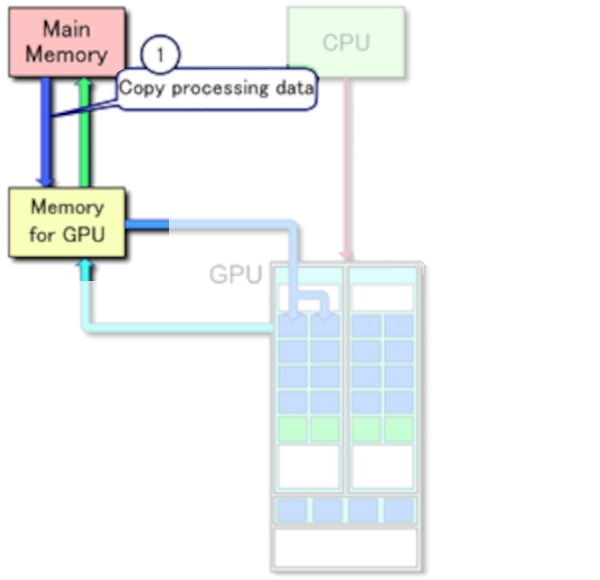
\includegraphics[width=\linewidth]{./figures/cuda_flow_memcpy}}
\end{frame}

\begin{frame}[fragile]{Copy $A$, $B$ to GPU}
    \begin{minted}[linenos,breaklines,firstnumber=109]{CUDA}
cudaMemcpy(a_gpu.data, a.data, a.rows * a.cols * sizeof(float), cudaMemcpyDefault);
cudaMemcpy(b_gpu.data, b.data, b.rows * b.cols * sizeof(float), cudaMemcpyDefault);
    \end{minted}

    \CUDA{cudaMemcpy(void *dst, const void *src, size_t bytes, cudaMemcpyKind kind)} copies \CUDA{bytes} bytes from \CUDA{src} to \CUDA{dst}.
    The final argument, \CUDA{kind}, specifies the direction. \\
    \onslide*<1>{On recent CUDA versions (CUDA 4+), this can be inferred using \CUDA{cudaMemcpyDefault}.}
    \onslide*<2>{
        On older CUDA versions, this should be one of
        \begin{itemize}
            \item \CUDA{cudaMemcpyHostToDevice}: CPU to GPU
            \item \CUDA{cudaMemcpyDeviceToHost}: GPU to CPU
            \item \CUDA{cudaMemcpyDeviceToDevice}: GPU to GPU
        \end{itemize}
    }

    \reminderImage{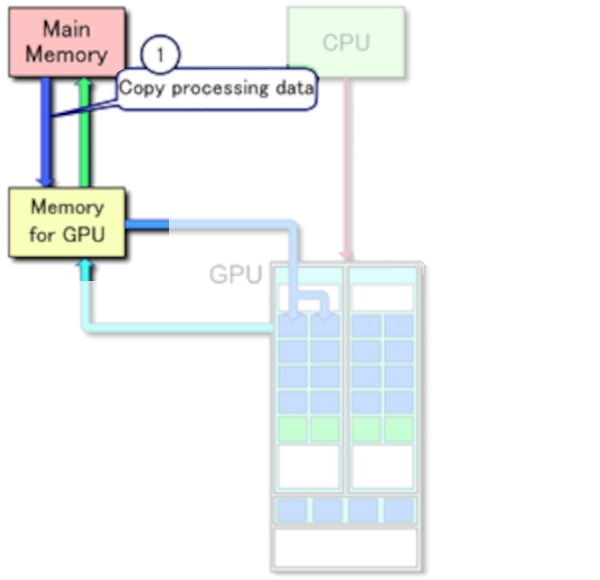
\includegraphics[width=\linewidth]{./figures/cuda_flow_memcpy}}
\end{frame}

\begin{frame}[fragile]{Start kernel}
    \begin{minted}[linenos,breaklines,firstnumber=7]{CUDA}
// TODO: we will implement this later
__global__ void matmul_gpu(matrix a, matrix b, matrix c);
    \end{minted}
    \CUDA{...}
    \begin{minted}[linenos,breaklines,firstnumber=112]{CUDA}
// specify grid (thread and block sizes)
dim3 threads = dim3(1024, 1024); // CUDA prefers powers of two
dim3 blocks = dim3(c.rows / 1024 + 1, c.cols / 1024 + 1);
// launch kernel
matmul_gpu<<<blocks, threads>>>(a_gpu, b_gpu, c_gpu);
cudaDeviceSynchronize();
    \end{minted}

    \onslide*<1> {
        The \CUDA{__global__} attribute specifies \CUDA{matmul_gpu} as a global (CPU to GPU) function. \\
        Recall that we had
        \begin{itemize}
            \item CPU-only (host) functions (using \CUDA{__host__})
            \item GPU-only (device) functions (using \CUDA{__device__})
            \item GPU to GPU entry point functions (using \CUDA{__global__})
        \end{itemize}
    }
    \onslide*<2> {
        \begin{itemize}
            \item Invoking global functions is always done by the \CUDA{<<<blocks, threads>>>} syntax.
            \item Make sure none of the arguments have pointers to CPU memory!
            \item Kernel launches are asynchronous, we use \CUDA{cudaDeviceSynchronize()} to have the CPU wait until the GPU is finished.
        \end{itemize}
    }

    \reminderImage{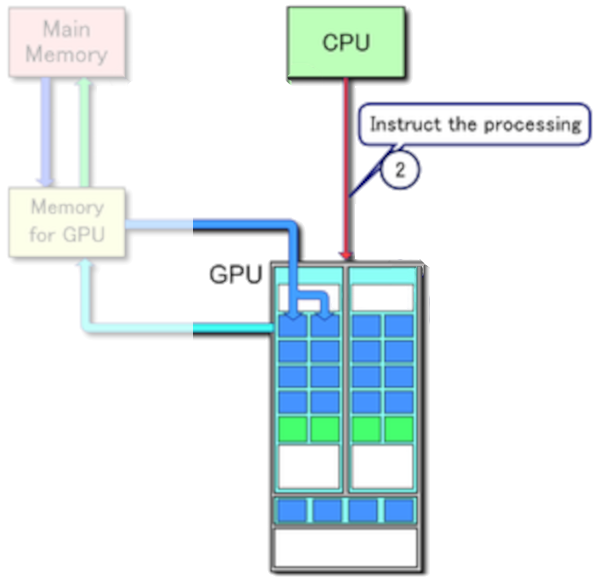
\includegraphics[width=\linewidth]{./figures/cuda_flow_launch}}
\end{frame}

\begin{frame}[fragile]{Copy $C$ to CPU}
    \begin{minted}[linenos,breaklines,firstnumber=118]{CUDA}
cudaMemcpy(c.data, c_gpu.data, c.rows * c.cols * sizeof(float), cudaMemcpyDefault);
    \end{minted}

    Same as before, \CUDA{cudaMemcpy(void *dst, const void *src, size_t size, cudaMemcpyKind kind)} copies data. \\
    Again, \CUDA{cudaMemcpyDefault} is used to infer direction (older systems should use \CUDA{cudaMemcpyDeviceToHost}).

    \reminderImage{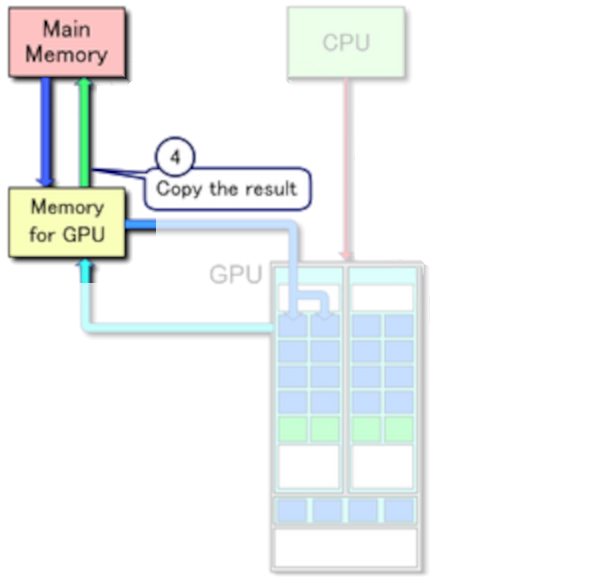
\includegraphics[width=\linewidth]{./figures/cuda_flow_memcpy_result}}
\end{frame}

\begin{frame}[fragile]{Implement kernel}
    \begin{minted}[linenos,breaklines]{CUDA}
struct matrix {
    __host__ __device__ float &at(int row, int col) {
        return data[row * cols + col];
    }
    float *data; int rows; int cols;
};
__host__ __device__ void dot(matrix a, matrix b, matrix c, int row, int col) {
    c.at(row, col) = 0;
    for(int k = 0; k < a.cols; k++)
        c.at(row, col) += a.at(row, k) * b.at(k, col);
}
    \end{minted}
    \begin{itemize}
        \item We will use \CUDA{matrix::at} and \CUDA{dot} on both CPU and GPU
        \item To avoid code duplication, we make the compiler generate both from one definition
        \begin{itemize}
            \item If we use \CUDA{__host__}, we only get CPU
            \item If we use \CUDA{__device__}, we only get GPU
            \item If we combine \CUDA{__host__ __device__}, we get both
        \end{itemize}
    \end{itemize}
    \reminderImage{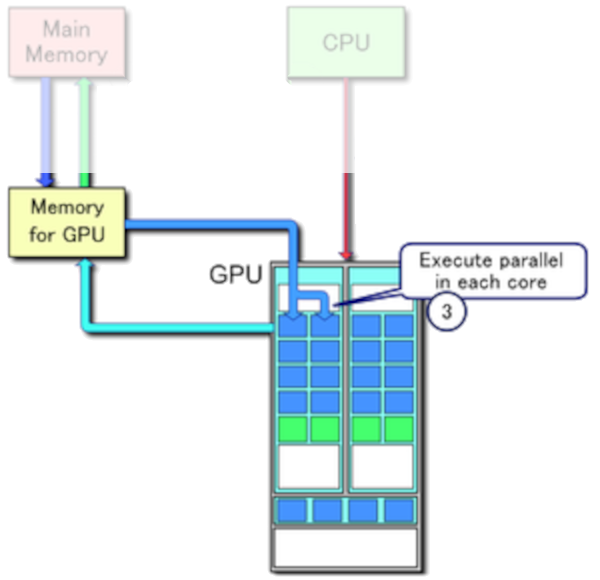
\includegraphics[width=\linewidth]{./figures/cuda_flow_kernel}}
\end{frame}

\begin{frame}[fragile]{Implement kernel}
    \begin{minted}[linenos,breaklines,firstnumber=7]{CUDA}
__global__ void matmul_gpu(matrix a, matrix b, matrix c) {
    int row = blockIdx.x * blockDim.x + threadIdx.x;
    int col = blockIdx.y * blockDim.y + threadIdx.y;
    if(row >= c.rows || col >= c.cols) // out-of-bounds
        return;

    dot(a, b, c, row, col);
}
    \end{minted}
    \begin{itemize}
        \item<only@1> \CUDA{matmul_gpu} has to be called from the CPU, but run on the GPU, so it should be \CUDA{__global__}
        \item<only@2> We launched $(\frac{\text{\CUDA{c.rows}}}{1024} + 1, \frac{\text{\CUDA{c.cols}}}{1024} + 1)$ blocks of $(1024, 1024)$ threads each
        \item<only@2> We can get indices using builtin variables:
        \begin{itemize}
            \item<only@2> \CUDA{threadIdx} holds the 3D thread index within a block
            \item<only@2> \CUDA{blockIdx} holds the 3D block index within the grid
            \item<only@2> \CUDA{blockDim} holds the 3D size of the block
        \end{itemize}
        \item<only@2> These indices can be out of bounds, so we need to check!
        \item<only@3> By making \CUDA{dot} (and \CUDA{matrix::at}) available on the GPU (using \CUDA{__device__}), we can simply re-use the code.
    \end{itemize}
    \reminderImage{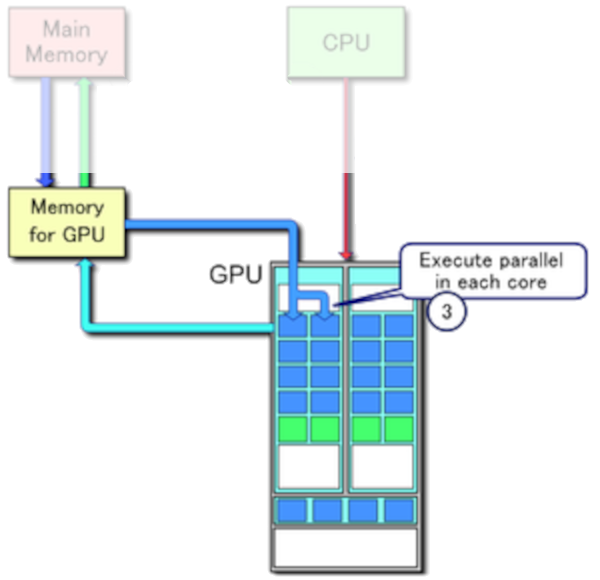
\includegraphics[width=\linewidth]{./figures/cuda_flow_kernel}}
\end{frame}

\begin{frame}[fragile]{Final code}
    \begin{minted}[linenos,breaklines]{CUDA}
struct matrix {
    __host__ __device__ float &at(int row, int col) {
        return data[row * cols + col];
    }
    float *data; int rows; int cols;
};
__host__ __device__ void dot(matrix a, matrix b, matrix c, int row, int col) {
    c.at(row, col) = 0;
    for(int k = 0; k < a.cols; k++)
        c.at(row, col) += a.at(row, k) * b.at(k, col);
}
__global__ void matmul_gpu(matrix a, matrix b, matrix c) {
    int row = blockIdx.x * blockDim.x + threadIdx.x;
    int col = blockIdx.y * blockDim.y + threadIdx.y;
    if(row >= c.rows || col >= c.cols) // out-of-bounds
        return;

    dot(a, b, c, row, col);
}
    \end{minted}
\end{frame}

\begin{frame}[fragile]{Final code}
    \begin{minted}[linenos,firstnumber=100,breaklines]{CUDA}
matrix a, b, c;
// Assume a, b, c are initialized
matrix a_gpu, b_gpu, c_gpu;
a_gpu.rows = a.rows; a_gpu.cols = a.cols;
cudaMalloc(&a_gpu.data, a.rows * a.cols * sizeof(float));
b_gpu.rows = b.rows; b_gpu.cols = b.cols;
cudaMalloc(&b_gpu.data, b.rows * b.cols * sizeof(float));
c_gpu.rows = c.rows; c_gpu.cols = c.cols;
cudaMalloc(&c_gpu.data, c.rows * c.cols * sizeof(float));
cudaMemcpy(a_gpu.data, a.data, a.rows * a.cols * sizeof(float), cudaMemcpyDefault);
cudaMemcpy(b_gpu.data, b.data, b.rows * b.cols * sizeof(float), cudaMemcpyDefault);
// specify grid (thread and block sizes)
dim3 threads = dim3(1024, 1024); // CUDA prefers powers of two
dim3 blocks = dim3(c.rows / 1024 + 1, c.cols / 1024 + 1);
// launch kernel
matmul_gpu<<<blocks, threads>>>(a_gpu, b_gpu, c_gpu);
cudaDeviceSynchronize();
cudaMemcpy(c.data, c_gpu.data, c.rows * c.cols * sizeof(float), cudaMemcpyDefault);
    \end{minted}
\end{frame}